\documentclass[a4paper,12pt]{report}

\usepackage[lmargin=2.00000cm,rmargin=2.0000cm,tmargin=5.5000cm,bmargin=2.500000cm,headheight=3.5cm]{geometry}        %Flexible and complete interface to document dimensions
\usepackage[utf8]{inputenc}
\usepackage[T1]{fontenc}
%\usepackage[latin1]{inputenc}
\usepackage{amsmath}
\usepackage{amsfonts}
\usepackage{amssymb}
\usepackage{lmodern}
\usepackage{float}
\usepackage{graphicx}

\usepackage[english,french]{babel}        %use for the below package `datetime'
\usepackage[babel=true]{csquotes}
\usepackage{datetime}        %Change format of `\today' with commands for current time
\renewcommand{\dateseparator}{-}
\newcommand{\headertoday}{\twodigit\day \dateseparator \twodigit\month  \dateseparator \the\year}

\usepackage{animate}
\usepackage{lastpage}
\usepackage{array}
\usepackage{lastpage}
\usepackage{multirow}
\usepackage{titling}
\usepackage{placeins}
\usepackage{media9}
\usepackage{eurosym}
\usepackage{pdflscape}
\usepackage{color}
\usepackage[table]{xcolor}
\definecolor{mon_bleu}{rgb}{0.137,0.466,0.741}
\definecolor{mon_vert}{rgb}{0.07843,0.4627,0.07843}
\definecolor{mon_rouge}{rgb}{0.62745,0.16078,0.27058}		
%\usepackage{subfigure}
\usepackage{subcaption}

\usepackage[ 
           hidelinks,
           colorlinks=true,
           linkcolor=blue,          % color of internal links (change box color with linkbordercolor)
    	   citecolor=blue,        % color of links to bibliography
    	   filecolor=blue,      % color of file links
    	   urlcolor=blue,           % color of external links
           pdfhighlight =/O]{hyperref}																		% dvipdfm package pour lien hypertextes dans pdf (pdfhighlight--> afficher la main dans le pdf, colorlinks--> colorlinks=true afficher les liens en couleurs)
  
\usepackage{blindtext}
\usepackage[final]{pdfpages}
\usepackage[french]{cleveref}																				% à placer après hyperref attention ne pas utiliser ":" dans les labels des équations avec French babel activé et cref

\usepackage{fancyhdr}
%%%%%%%%%%%%%%%%%%%%%%%%%%%%%%%%%%%%%%%%%%%%%%%%%%%%%%%%%%%%%%%%%%%%%%%%%%
%                         FORMAT PERSONNALISES                           %
% %%%%%%%%%%%%%%%%%%%%%%%%%%%%%%%%%%%%%%%%%%%%%%%%%%%%%%%%%%%%%%%%%%%%%%%%

\parindent=0pt        %leading space for paragraphs
\pagestyle{fancy}
\renewcommand{\arraystretch}{1.5}
\renewcommand{\headrulewidth}{0pt}
\fancyhead[CE,CO,LE,LO,RE,RO]{} %% clear out all headers
\fancyhead[C]{%
\begin{tabular}{|m{3.0cm}|m{10cm}|c@{}|}
\hline
\multirow{2}{*}{\includegraphics[scale=0.045]																			% LOGO LABO
{Logo-Symme.png}}& \centering \multirow{2}{*}{ \Large{\thetitle}}  &  \multirow{2}{*}{Page: \thepage ~/ \pageref{LastPage}}\\
& &  \\
\hline
%Etabli par: \newline \theauthor & \multicolumn{2}{l|}{Diffusion: interne}\\
%\hline
\multicolumn{2}{|l|}{Objet: \thetitleobject }& Date: \headertoday ~~\\ 
\hline
\end{tabular}
}
\renewcommand\footrulewidth{1pt}
\fancyfoot[L]{Document confidentiel} 																		% DOCUMENT CONFIDENTIEL
\fancyfoot[R]{Laboratoire SYMME}		 																	% NOM DU LABO

\newcolumntype{x}[1]{>{\centering\hspace{0pt}}p{#1}}
\setlength{\doublerulesep}{\arrayrulewidth} 


\usepackage{tikz}																							% pour les diagrammes
\usetikzlibrary{calc}
\usetikzlibrary{shapes.geometric,shapes.arrows,decorations.pathmorphing}
\usetikzlibrary{matrix,chains,scopes,positioning,shapes,arrows,fit}
\usetikzlibrary{calc,decorations.pathreplacing}
\usetikzlibrary{calc}
\usetikzlibrary{backgrounds,decorations.markings}

\setcounter{secnumdepth}{5}		%sous sous sous section



%%%%%%%%%%%%%%%%%%%%%%%%%%%%%%%%%%%%%%%%%%%%%%%%%%%%%%%%%%%%%%%%%%%%%%%%%%%%%%%%%%%%
%%-------------> PAGE DE GARDE INFO
%%%%%%%%%%%%%%%%%%%%%%%%%%%%%%%%%%%%%%%%%%%%%%%%%%%%%%%%%%%%%%%%%%%%%%%%%%%%%%%%%%%%

\author{Auteur}
\newcommand{\validator}{J. COLLOMB}
\title{Rapport d'avancement}
\selectlanguage{french}	
\date{\today}
\newcommand{\thetitleobject}{Comment intégrer une animation ?}
\setcounter{tocdepth}{6}
\setcounter{secnumdepth}{6}


%%%%%%%%%%%%%%%%%%%%%%%%%%%%%%%%%%%%%%%%%%%%%%%%%%%%%%%%%%%%%%%%%%%%%%%%%%%%%%%%%%%%
%%-------------> DEBUT DU DOCUMENT 
%%%%%%%%%%%%%%%%%%%%%%%%%%%%%%%%%%%%%%%%%%%%%%%%%%%%%%%%%%%%%%%%%%%%%%%%%%%%%%%%%%%%

\begin{document}

\graphicspath{{Figures/}}

%%%%%%%%%%%%%%%%%%%%%%%%%%%%%%%%%%%%%%%%%%%%%%%%%%%%%%%%%%%%%%%%%%%%%%%%%%%%%%%%%%%%
%%-------------> PAGE DE GARDE 
%%%%%%%%%%%%%%%%%%%%%%%%%%%%%%%%%%%%%%%%%%%%%%%%%%%%%%%%%%%%%%%%%%%%%%%%%%%%%%%%%%%%
\begin{titlepage}
    \centering
    \vspace*{3cm}
    {\bfseries\Large
        \thetitle\\
        \thetitleobject\\
        --- \\
        Document confidentiel\\  																			% LIGNE "CONFIDENTIEL"
        \vskip2cm
    }
    
\includegraphics[scale=0.65]{logos.png}  																% LOGOS DES PARTENAIRES
    \vfill
    \begin{center}
    \begin{table}[b]
    \begin{tabular}{x{.225\linewidth}|| x{.225\linewidth}|| x{.225\linewidth} || x{.225\linewidth} }
    \hline \hline
    \textbf{Date} & \textbf{Révision} & \textbf{Rédigé par} & \textbf{Validé par} \tabularnewline
    \hline \hline
    \thedate & Rev. A  &  \theauthor &  \validator \tabularnewline
    \hline
    ~ & ~ & ~ & ~ \tabularnewline
    \hline
    ~ & ~ & ~ & ~ \tabularnewline
    \hline
    ~ & ~ & ~ & ~\tabularnewline         
    \hline \hline                                                                   
    \end{tabular}
    \end{table}
    \end{center}
    \vfill
    \vfill
    \begin{tikzpicture}[remember picture,overlay]
    \node (label) at (8cm,20cm){
        
\includegraphics[width=2.5cm]{Logo-Symme.png} 													% LOGO LABO
      };
    
	\draw[very thick]
		([yshift=-25pt,xshift=25pt]current page.north west)--
		([yshift=-25pt,xshift=-25pt]current page.north east)--
		([yshift=25pt,xshift=-25pt]current page.south east)--
		([yshift=25pt,xshift=25pt]current page.south west)--cycle;
    \end{tikzpicture}
\end{titlepage}


%\begin{titlepage}
%    \centering
%    
%    \vspace*{3cm}
%    {\bfseries\Large
%        \thetitle\\
%        \thetitleobject\\
%        \vskip2cm
%    }    
%    \vfill
%    \begin{center}
%    \begin{table}[b]
%    \begin{tabular}{x{.225\linewidth}|| x{.225\linewidth}|| x{.225\linewidth} || x{.225\linewidth} }
%    \hline \hline
%    \textbf{Date} & \textbf{R�vision} & \textbf{R�dig� par} & \textbf{Valid� par} \tabularnewline
%    \hline \hline
%    \thedate & Rev. A  &  \theauthor &  \validator \tabularnewline
%    \hline
%    ~ & ~ & ~ & ~ \tabularnewline
%    \hline
%    ~ & ~ & ~ & ~ \tabularnewline
%    \hline
%    ~ & ~ & ~ & ~\tabularnewline         
%    \hline \hline                                                                   
%    \end{tabular}
%    \end{table}
%    \end{center}
%    \vfill
%    \vfill
%    \begin{tikzpicture}[overlay,remember picture]
%    \node (label) at (6.7cm,19.5cm){
%        \includegraphics[width=4cm]{../Figures/logo_CT1.pdf} % also works with logo.pdf
%      };
%    
%    \draw [line width=1pt,rounded corners=7pt]
%        ($ (current page.north west) + (1.5cm,-1.5cm) $)
%        rectangle
%        ($ (current page.south east) + (-1.5cm,1.5cm) $);
%        
%%	\draw[very thick]
%%		([yshift=-25pt,xshift=25pt]current page.north west)--
%%		([yshift=-25pt,xshift=-25pt]current page.north east)--
%%		([yshift=25pt,xshift=-25pt]current page.south east)--
%%		([yshift=25pt,xshift=25pt]current page.south west)--cycle;
%    \end{tikzpicture}
%\end{titlepage}


%%%%%%%%%%%%%%%%%%%%%%%%%%%%%%%%%%%%%%%%%%%%%%%%%%%%%%%%%%%%%%%%%%%%%%%%%%%%%%%%%%%%
%%-------------> SOMMAIRE
%%%%%%%%%%%%%%%%%%%%%%%%%%%%%%%%%%%%%%%%%%%%%%%%%%%%%%%%%%%%%%%%%%%%%%%%%%%%%%%%%%%%

\renewcommand\contentsname{Sommaire}
\setcounter{chapter}{1}
\tableofcontents
%\listoffigures
%\listoftables


%%%%%%%%%%%%%%%%%%%%%%%%%%%%%%%%%%%%%%%%%%%%%%%%%%%%%%%%%%%%%%%%%%%%%%%%%%%%%%%%%%%%
%%-------------> CORPS DOCUMENT
%%%%%%%%%%%%%%%%%%%%%%%%%%%%%%%%%%%%%%%%%%%%%%%%%%%%%%%%%%%%%%%%%%%%%%%%%%%%%%%%%%%%

%-----------------------------------------------------------------------------------
%-----------------------------------------------------------------------------------
\newpage

\section{Préparation amont}
\subsection{Principe}
Tout comme les films, une animation est générée par l'assemblage de plusieurs images à une cadence plus ou moins importante. Une animation fluide possède une fréquence de l'ordre de 25 images/seconde, mais pour certaines applications, des fréquences inférieures ou supérieures peuvent être requises.

\subsection{Génération des images}
Les images peuvent être générées de différentes manières :
\begin{itemize}
\item sous Python/Matlab\ldots;
\item sous logiciel éléments finis;
\item \ldots
\end{itemize}

Pour un bon fonctionnement sous \LaTeX, il est nécessaire de nommer les fichiers sous un format du type : \verb|nom_du_fichier_1.pdf| ; \verb|nom_du_fichier_2.pdf| ; \ldots

\begin{figure}[hbtp]
	\centering
	\begin{subfigure}[b]{0.25\textwidth}
		\centering
		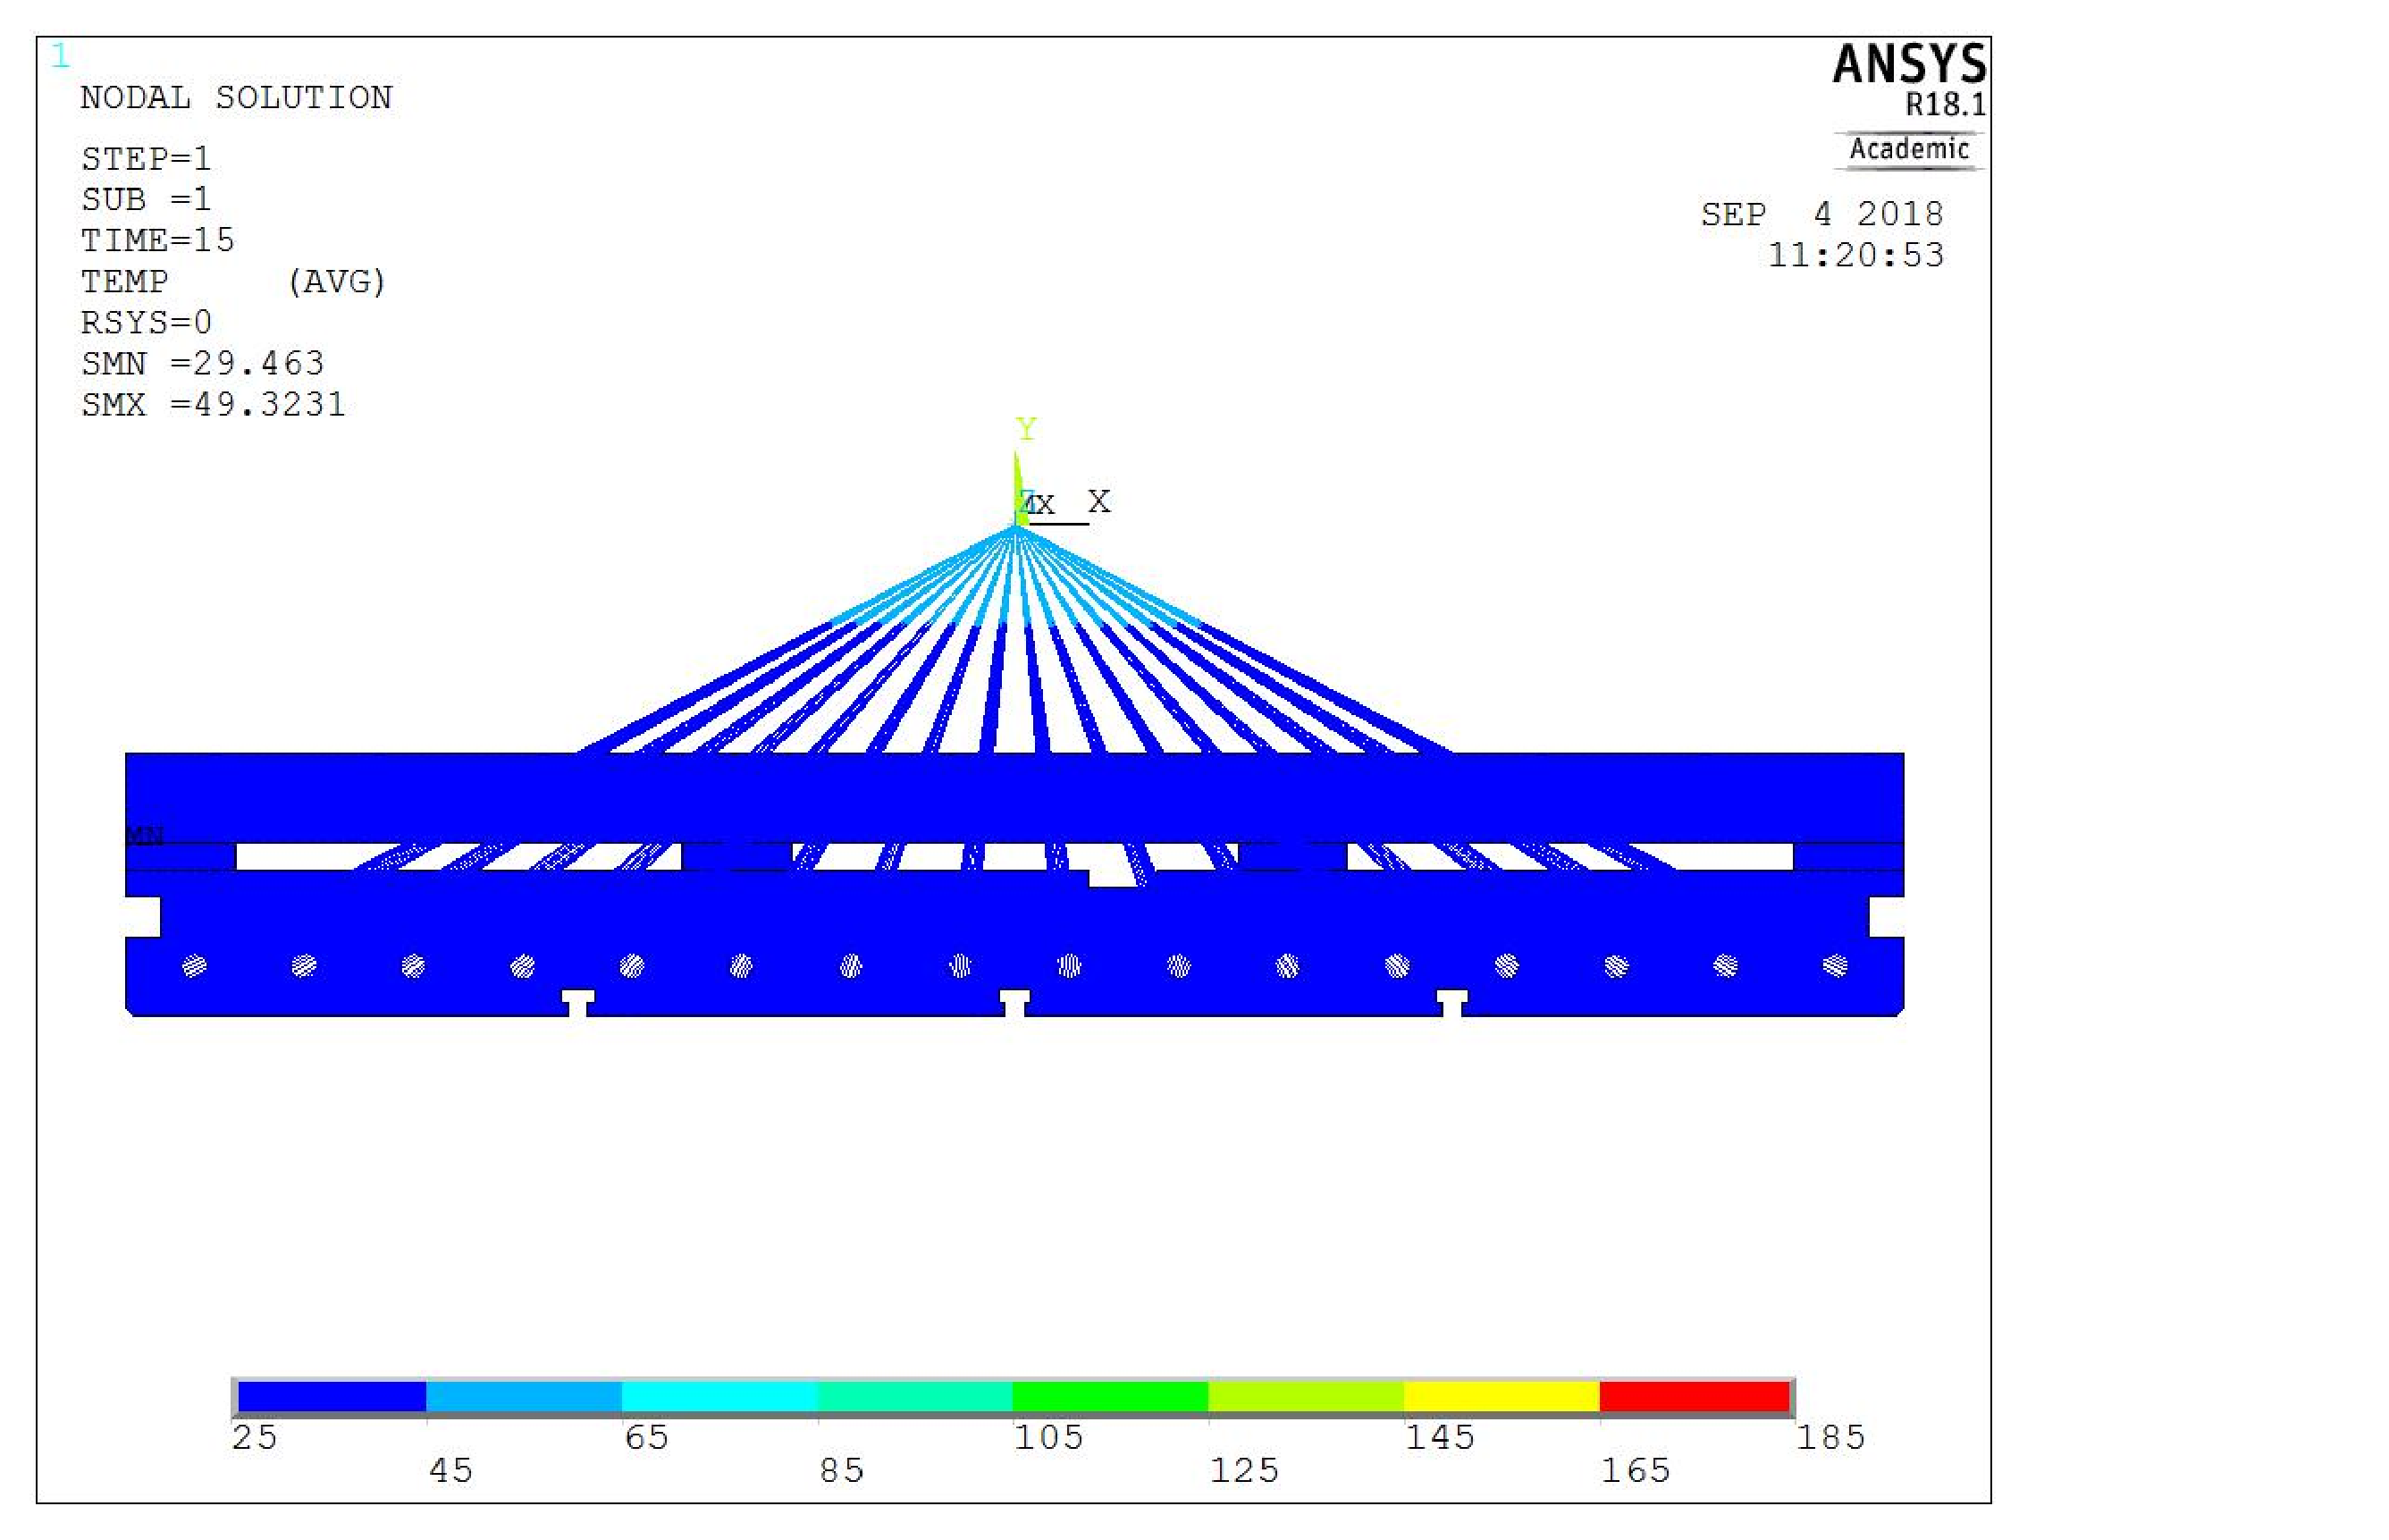
\includegraphics[scale=0.12]{Figures/animation/Figure_1.pdf}
	\end{subfigure}
	\qquad
	\begin{subfigure}[b]{0.25\textwidth}
		\centering
		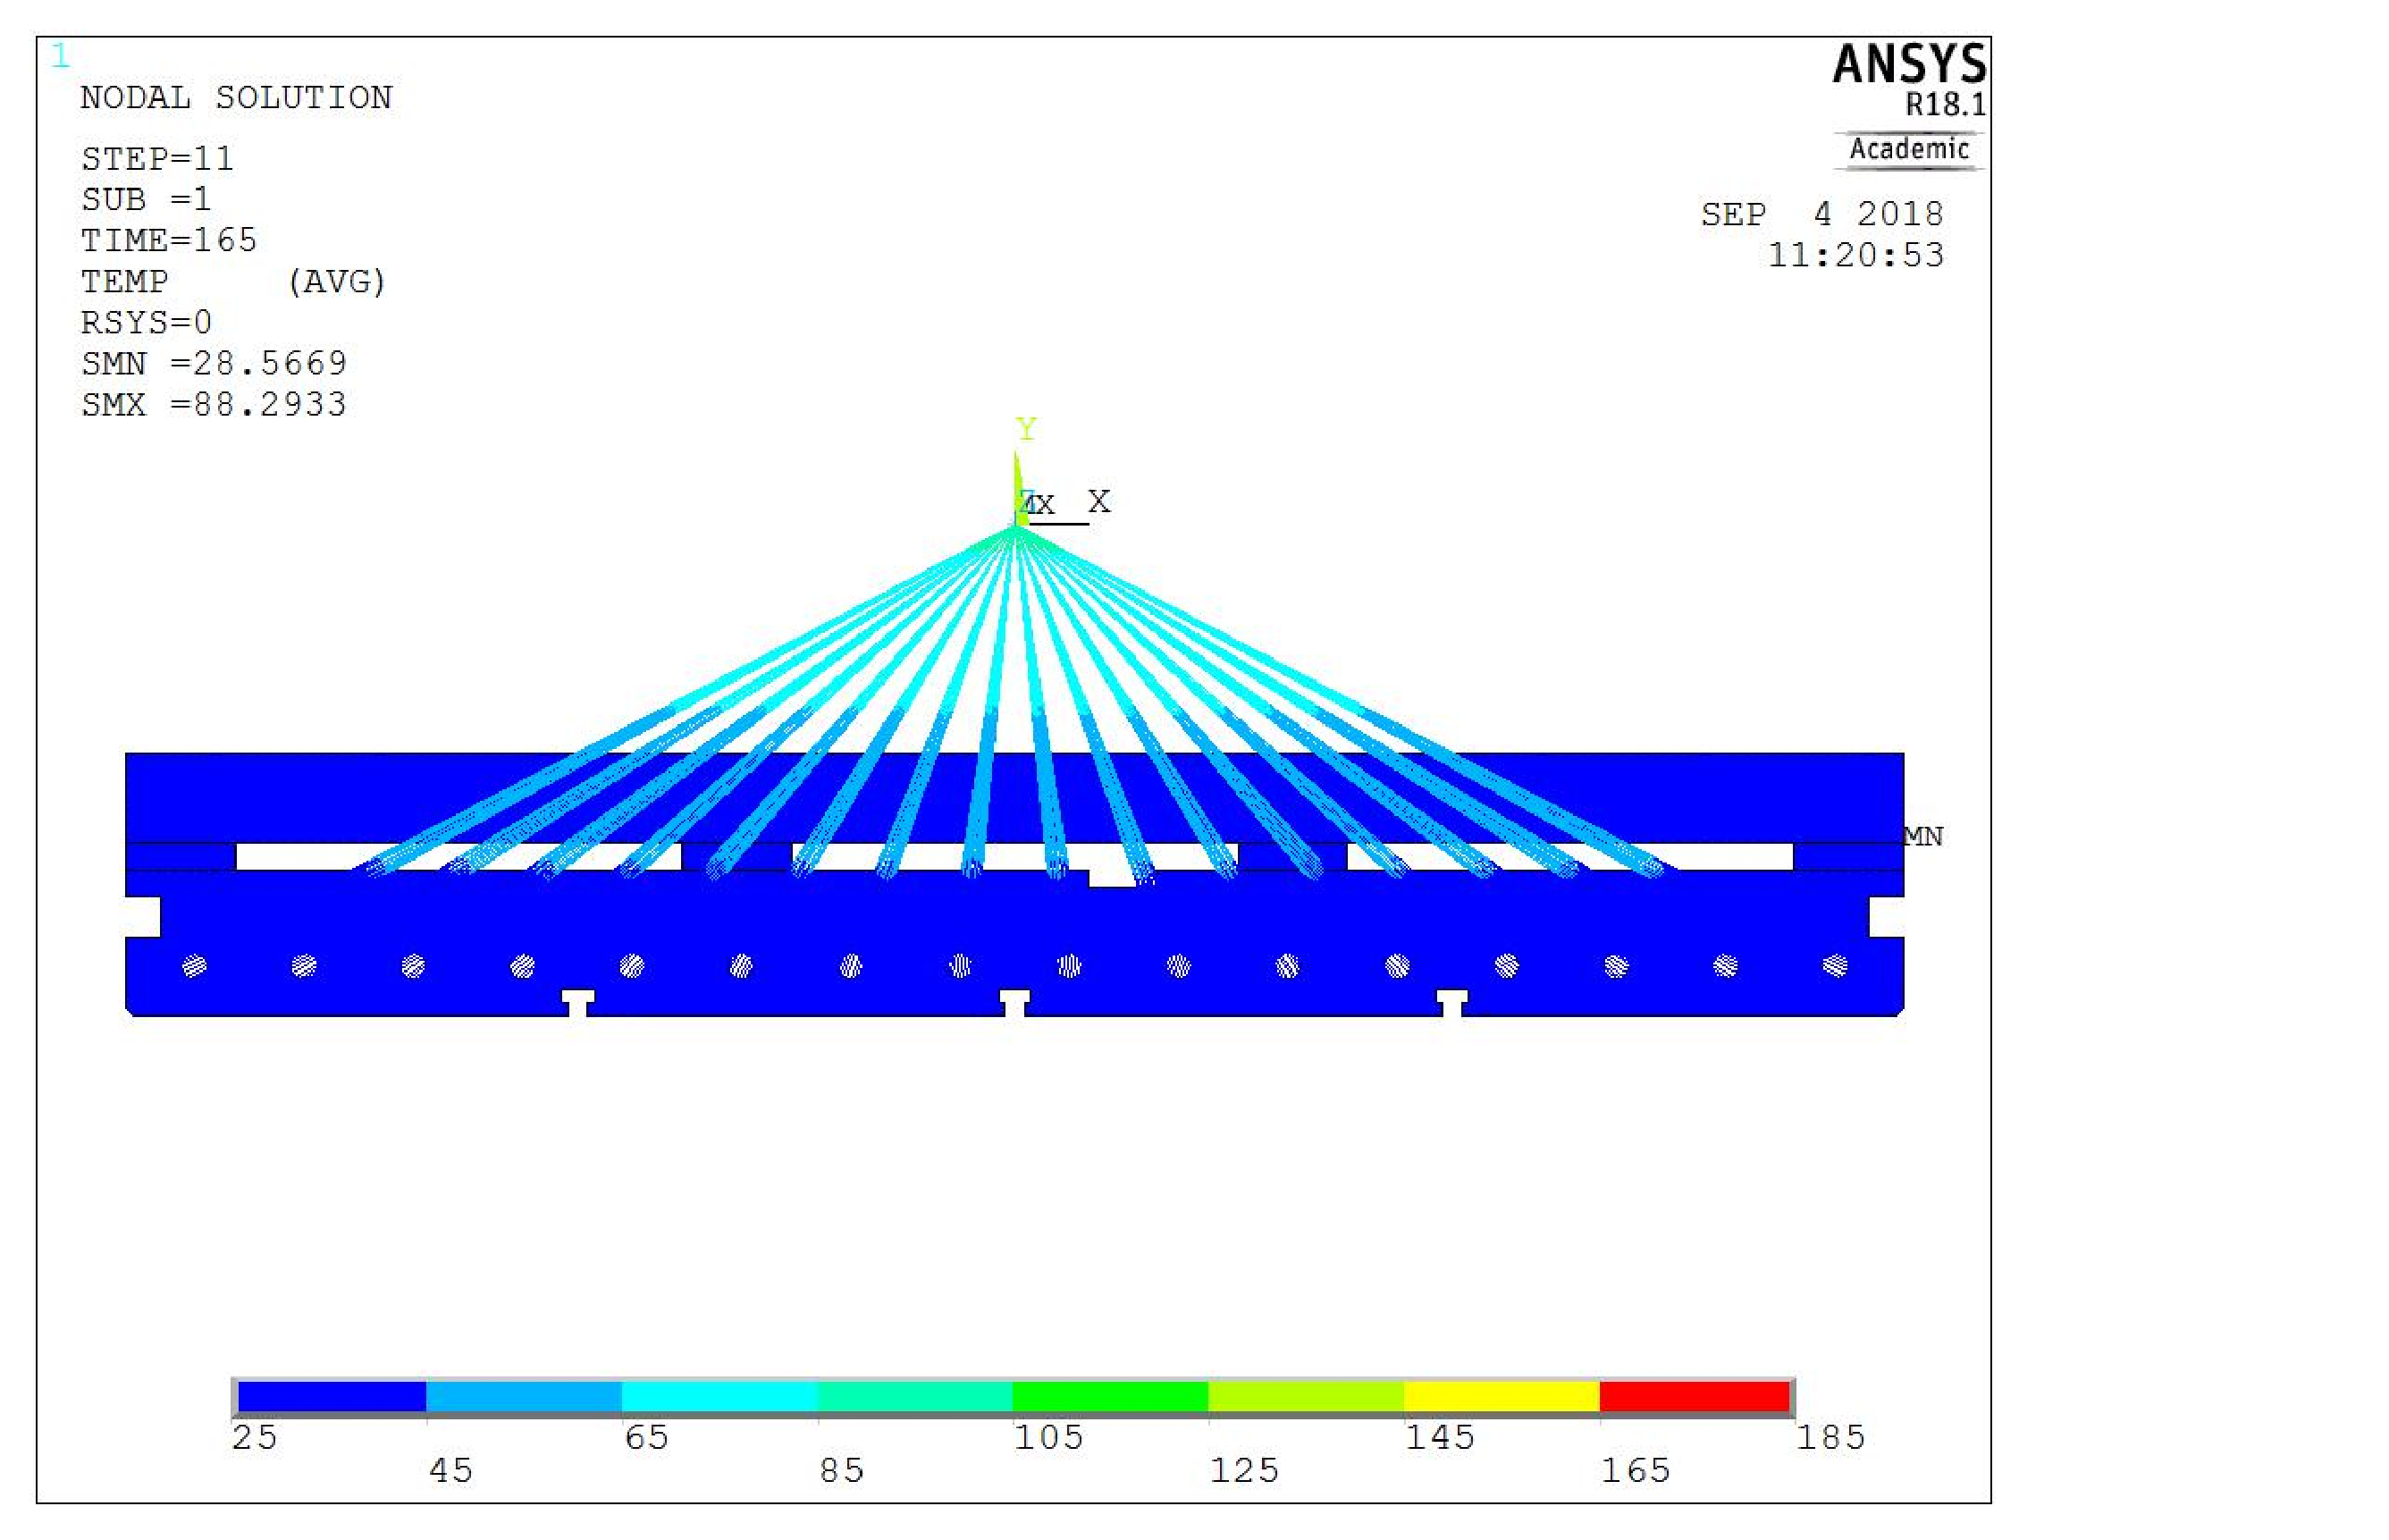
\includegraphics[scale=0.12]{Figures/animation/Figure_3.pdf}
	\end{subfigure}
	\qquad
	\begin{subfigure}[b]{0.25\textwidth}
		\centering
		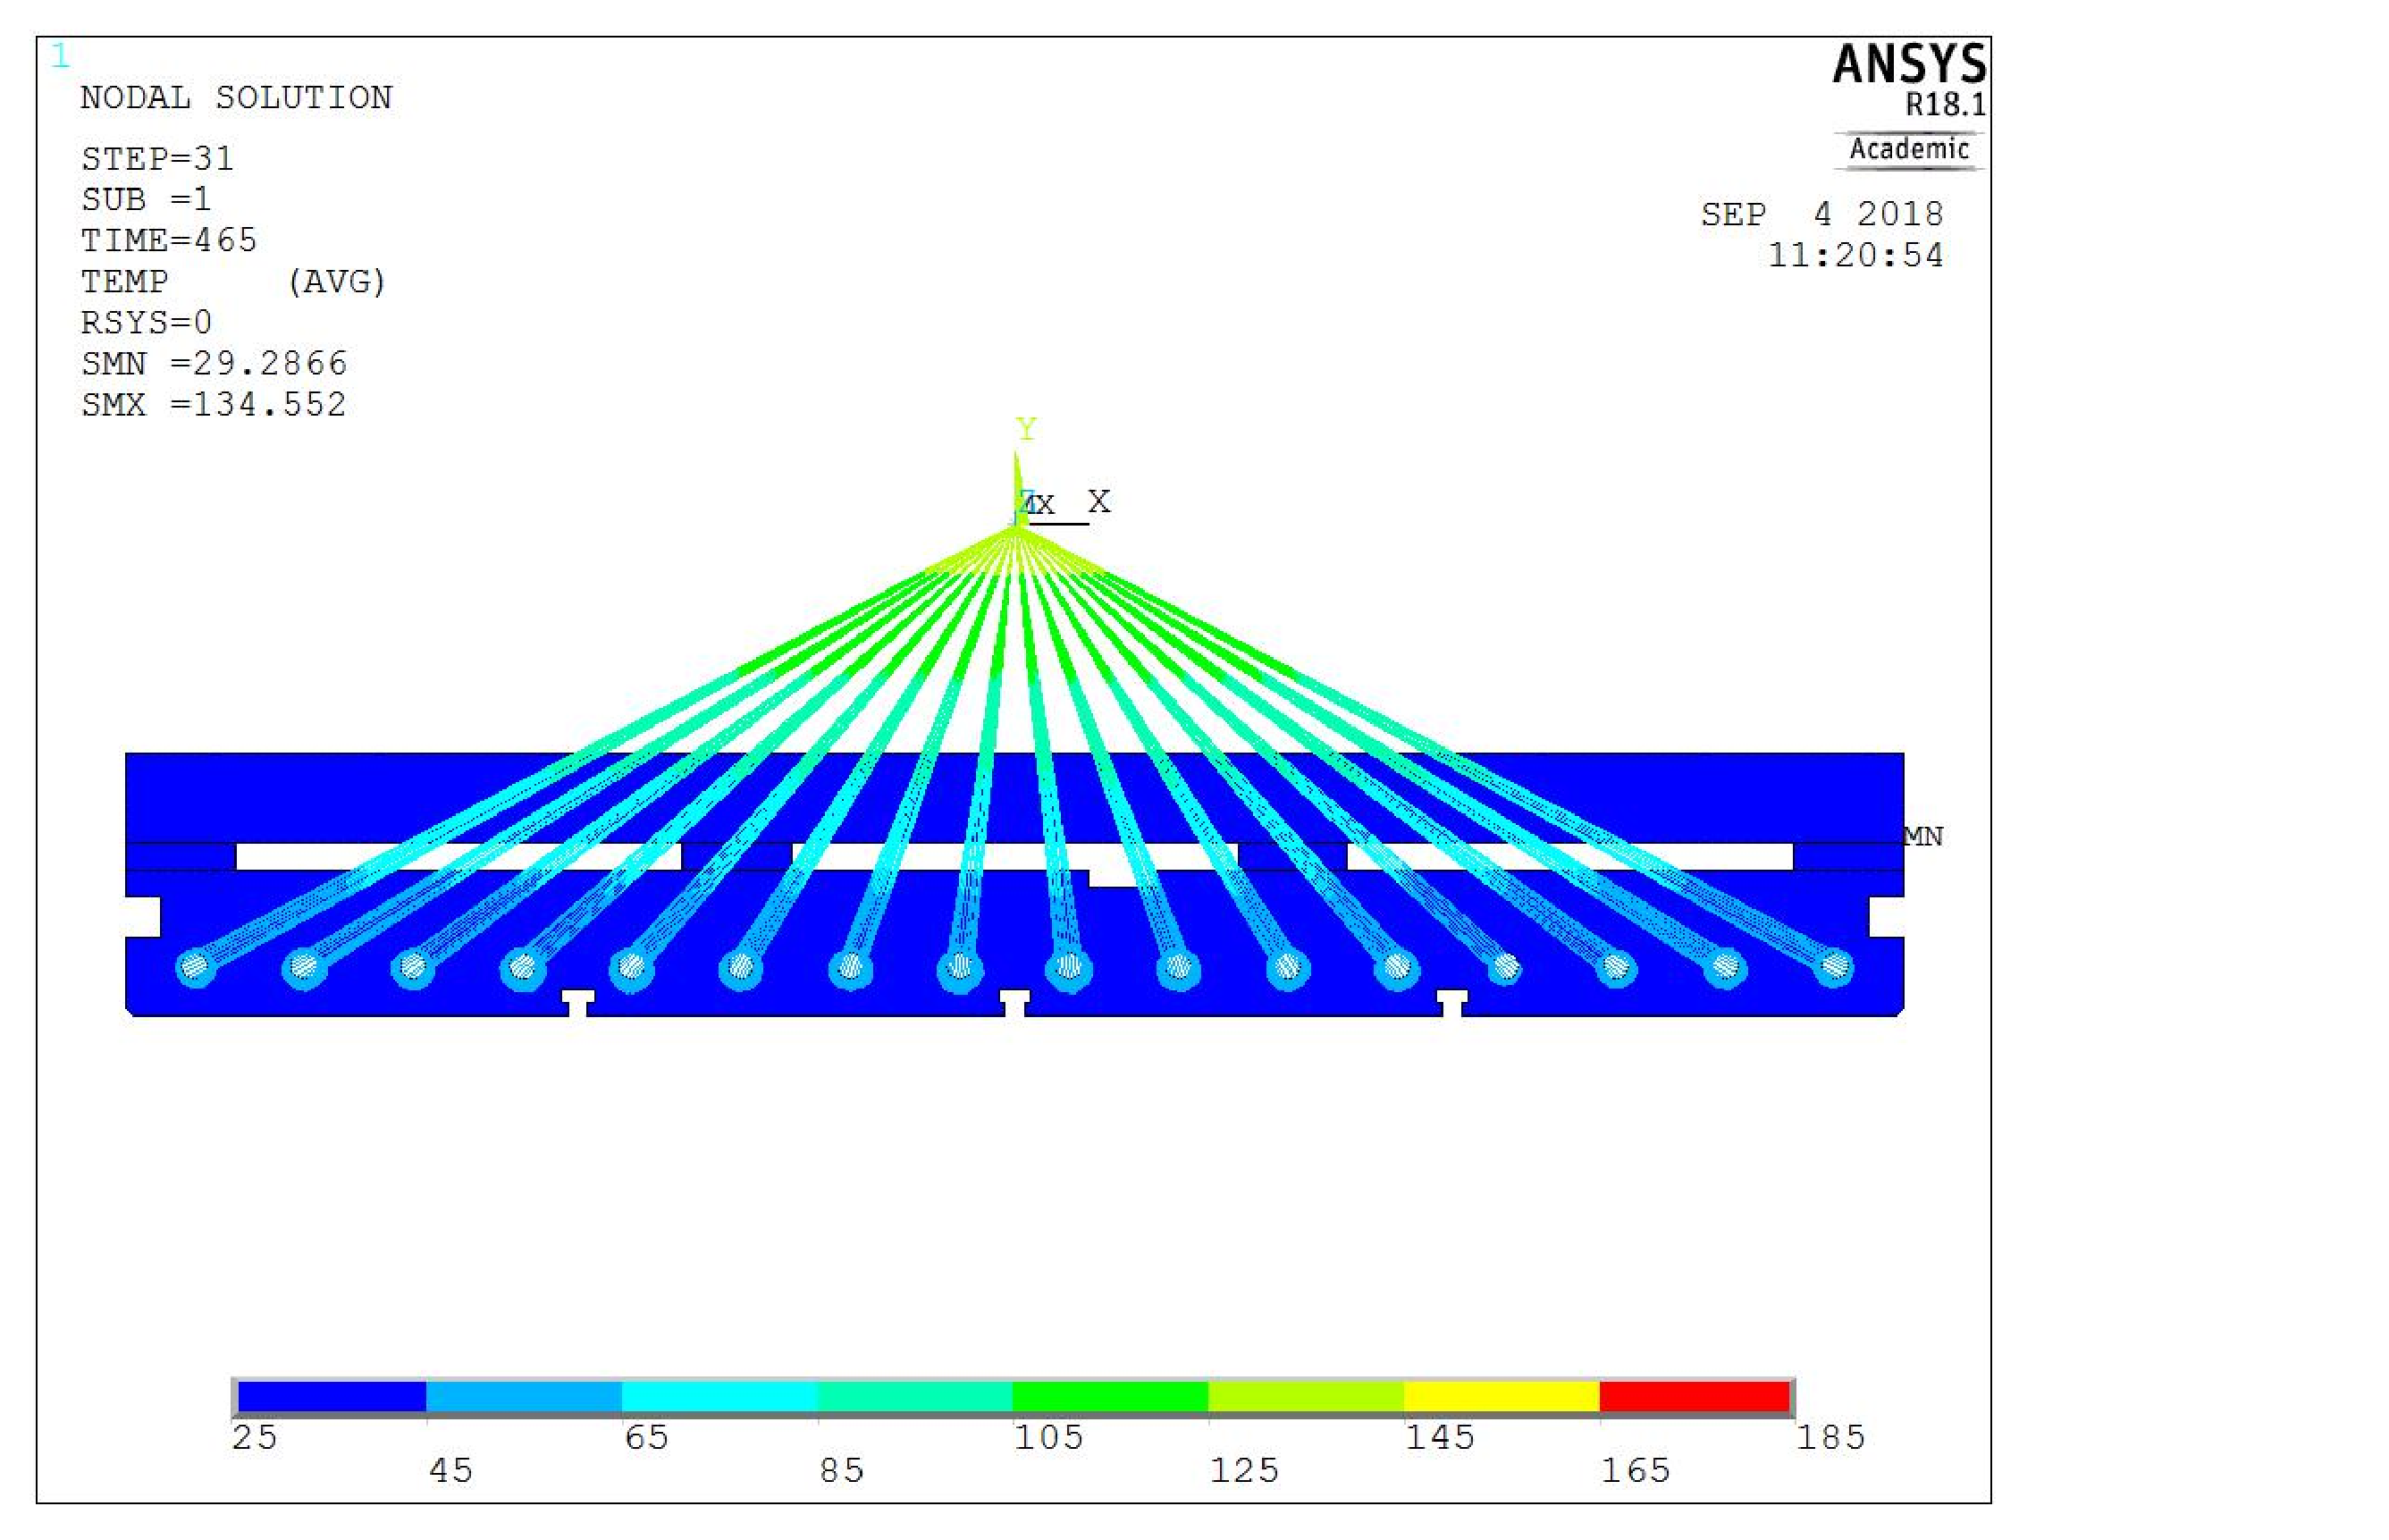
\includegraphics[scale=0.12]{Figures/animation/Figure_5.pdf}
	\end{subfigure}
	\qquad
	\begin{subfigure}[b]{0.25\textwidth}
		\centering
		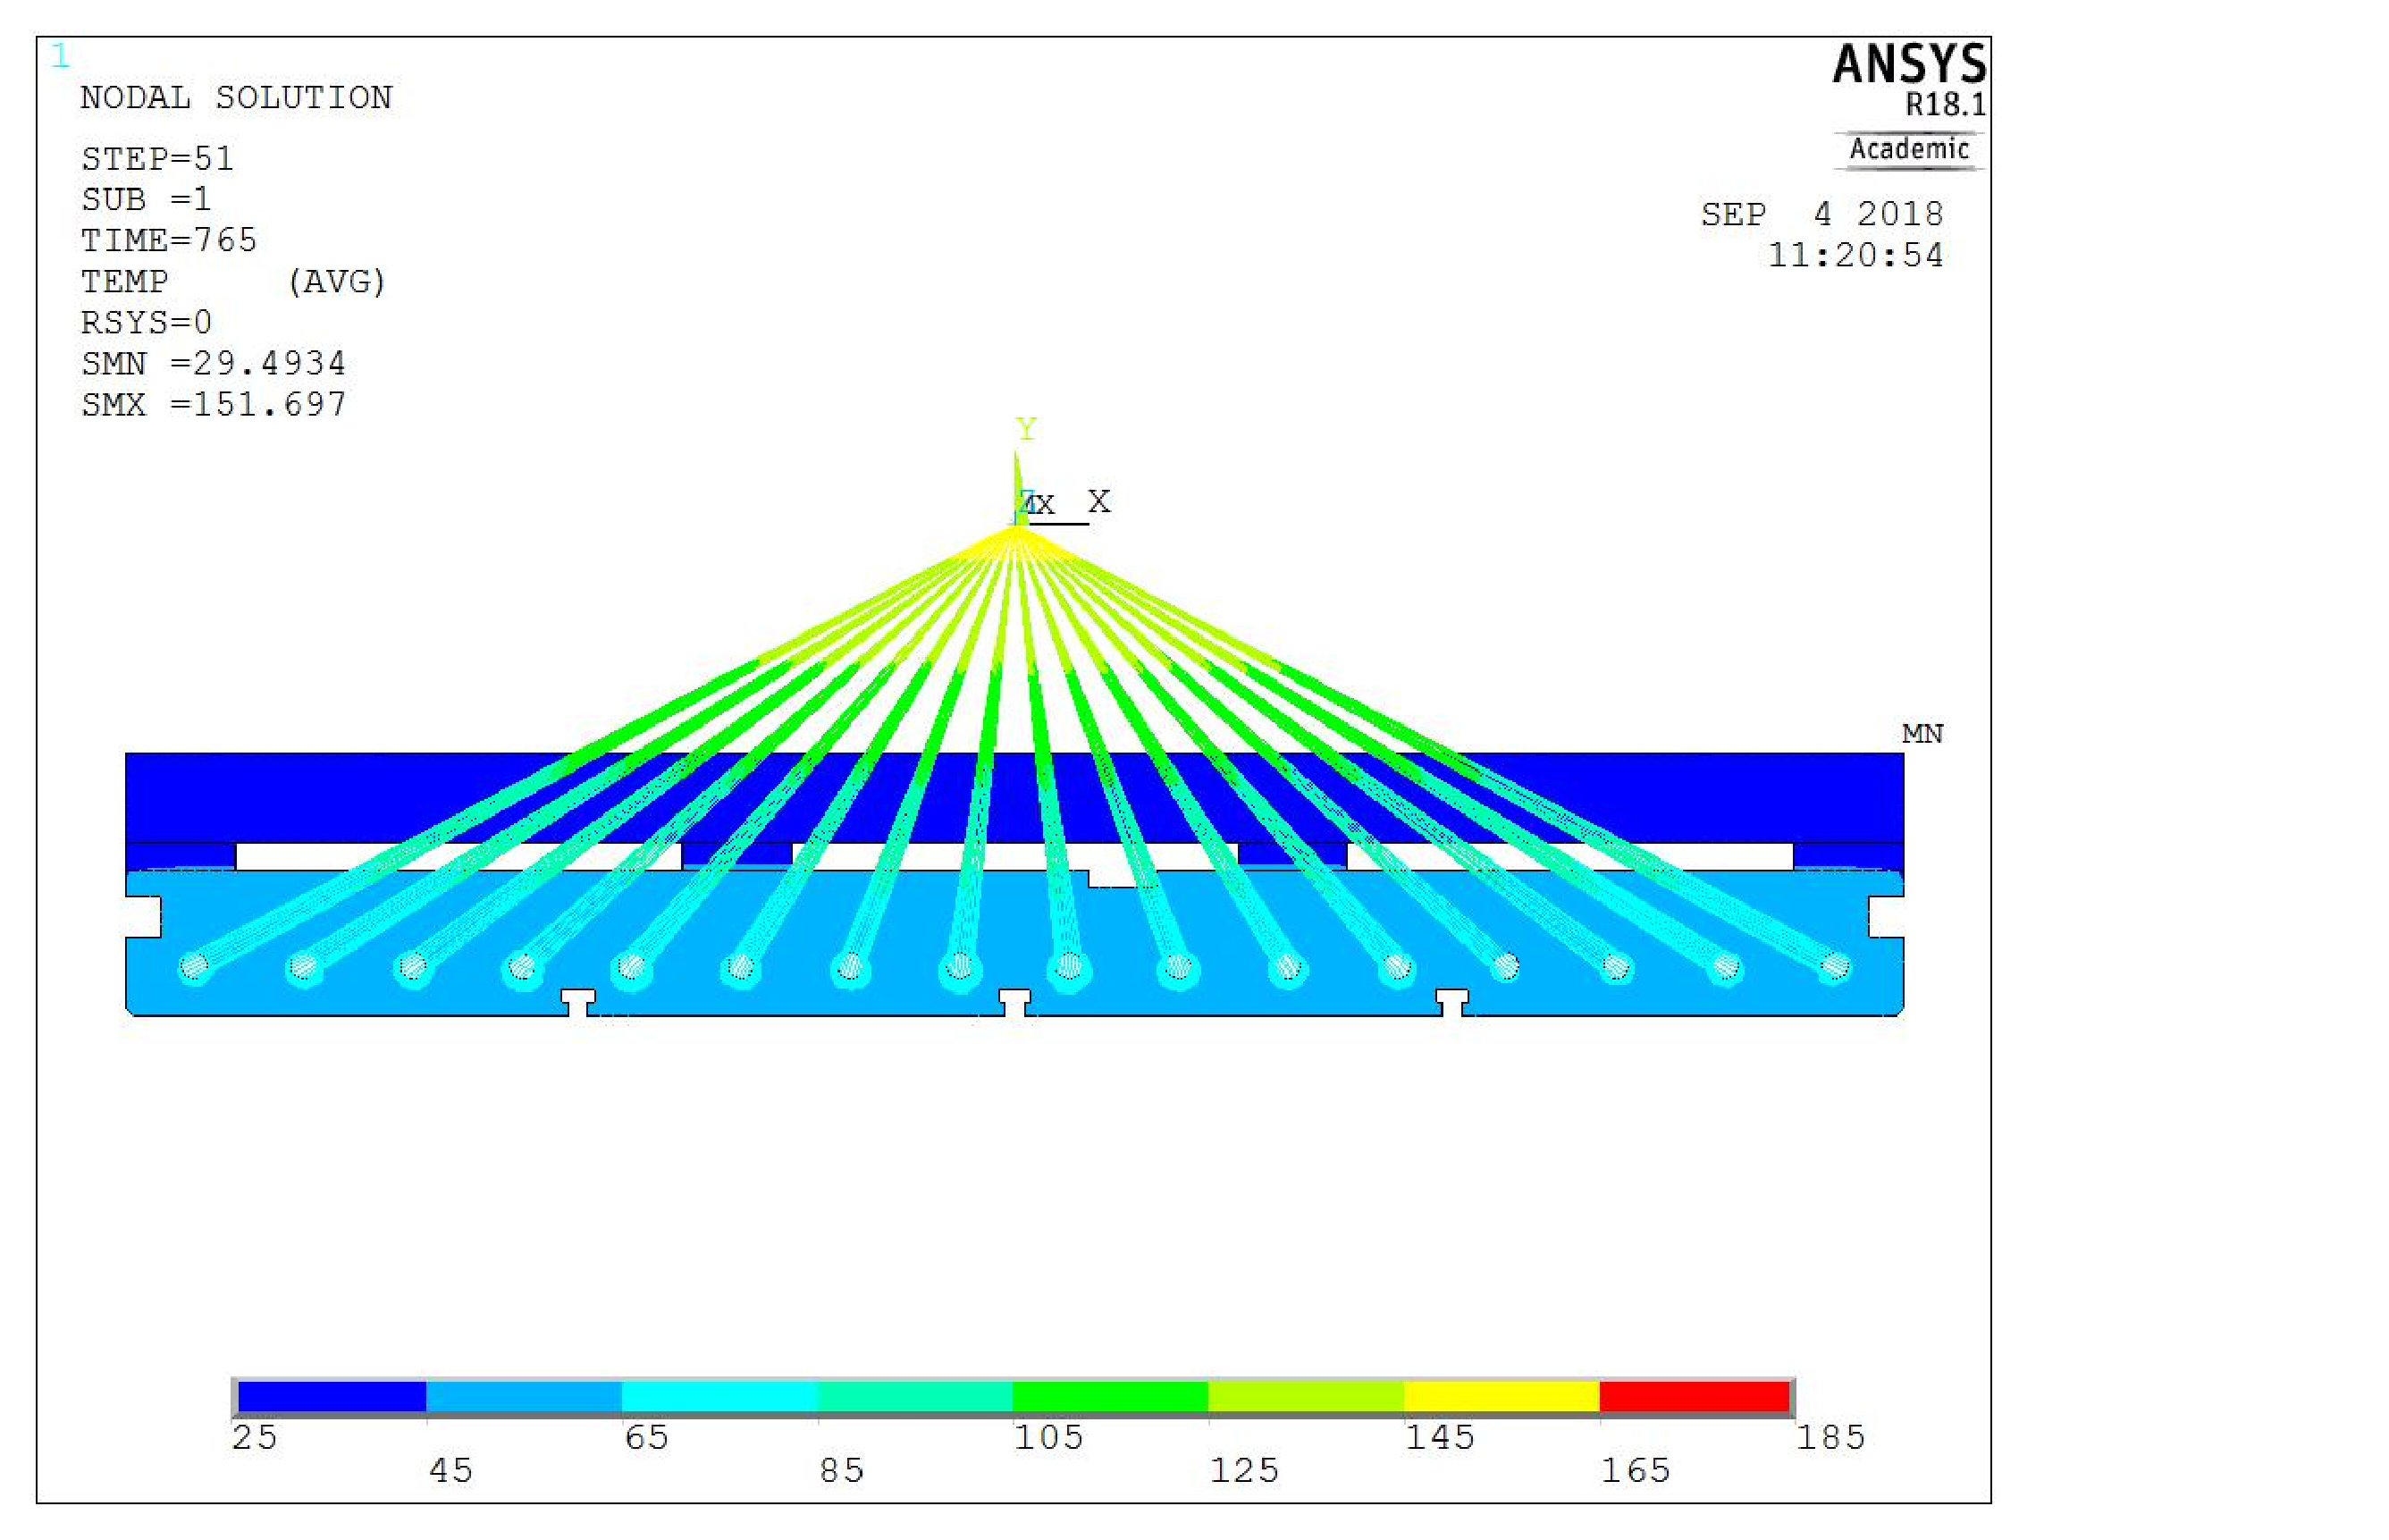
\includegraphics[scale=0.12]{Figures/animation/Figure_7.pdf}
	\end{subfigure}
	\qquad
	\begin{subfigure}[b]{0.25\textwidth}
		\centering
		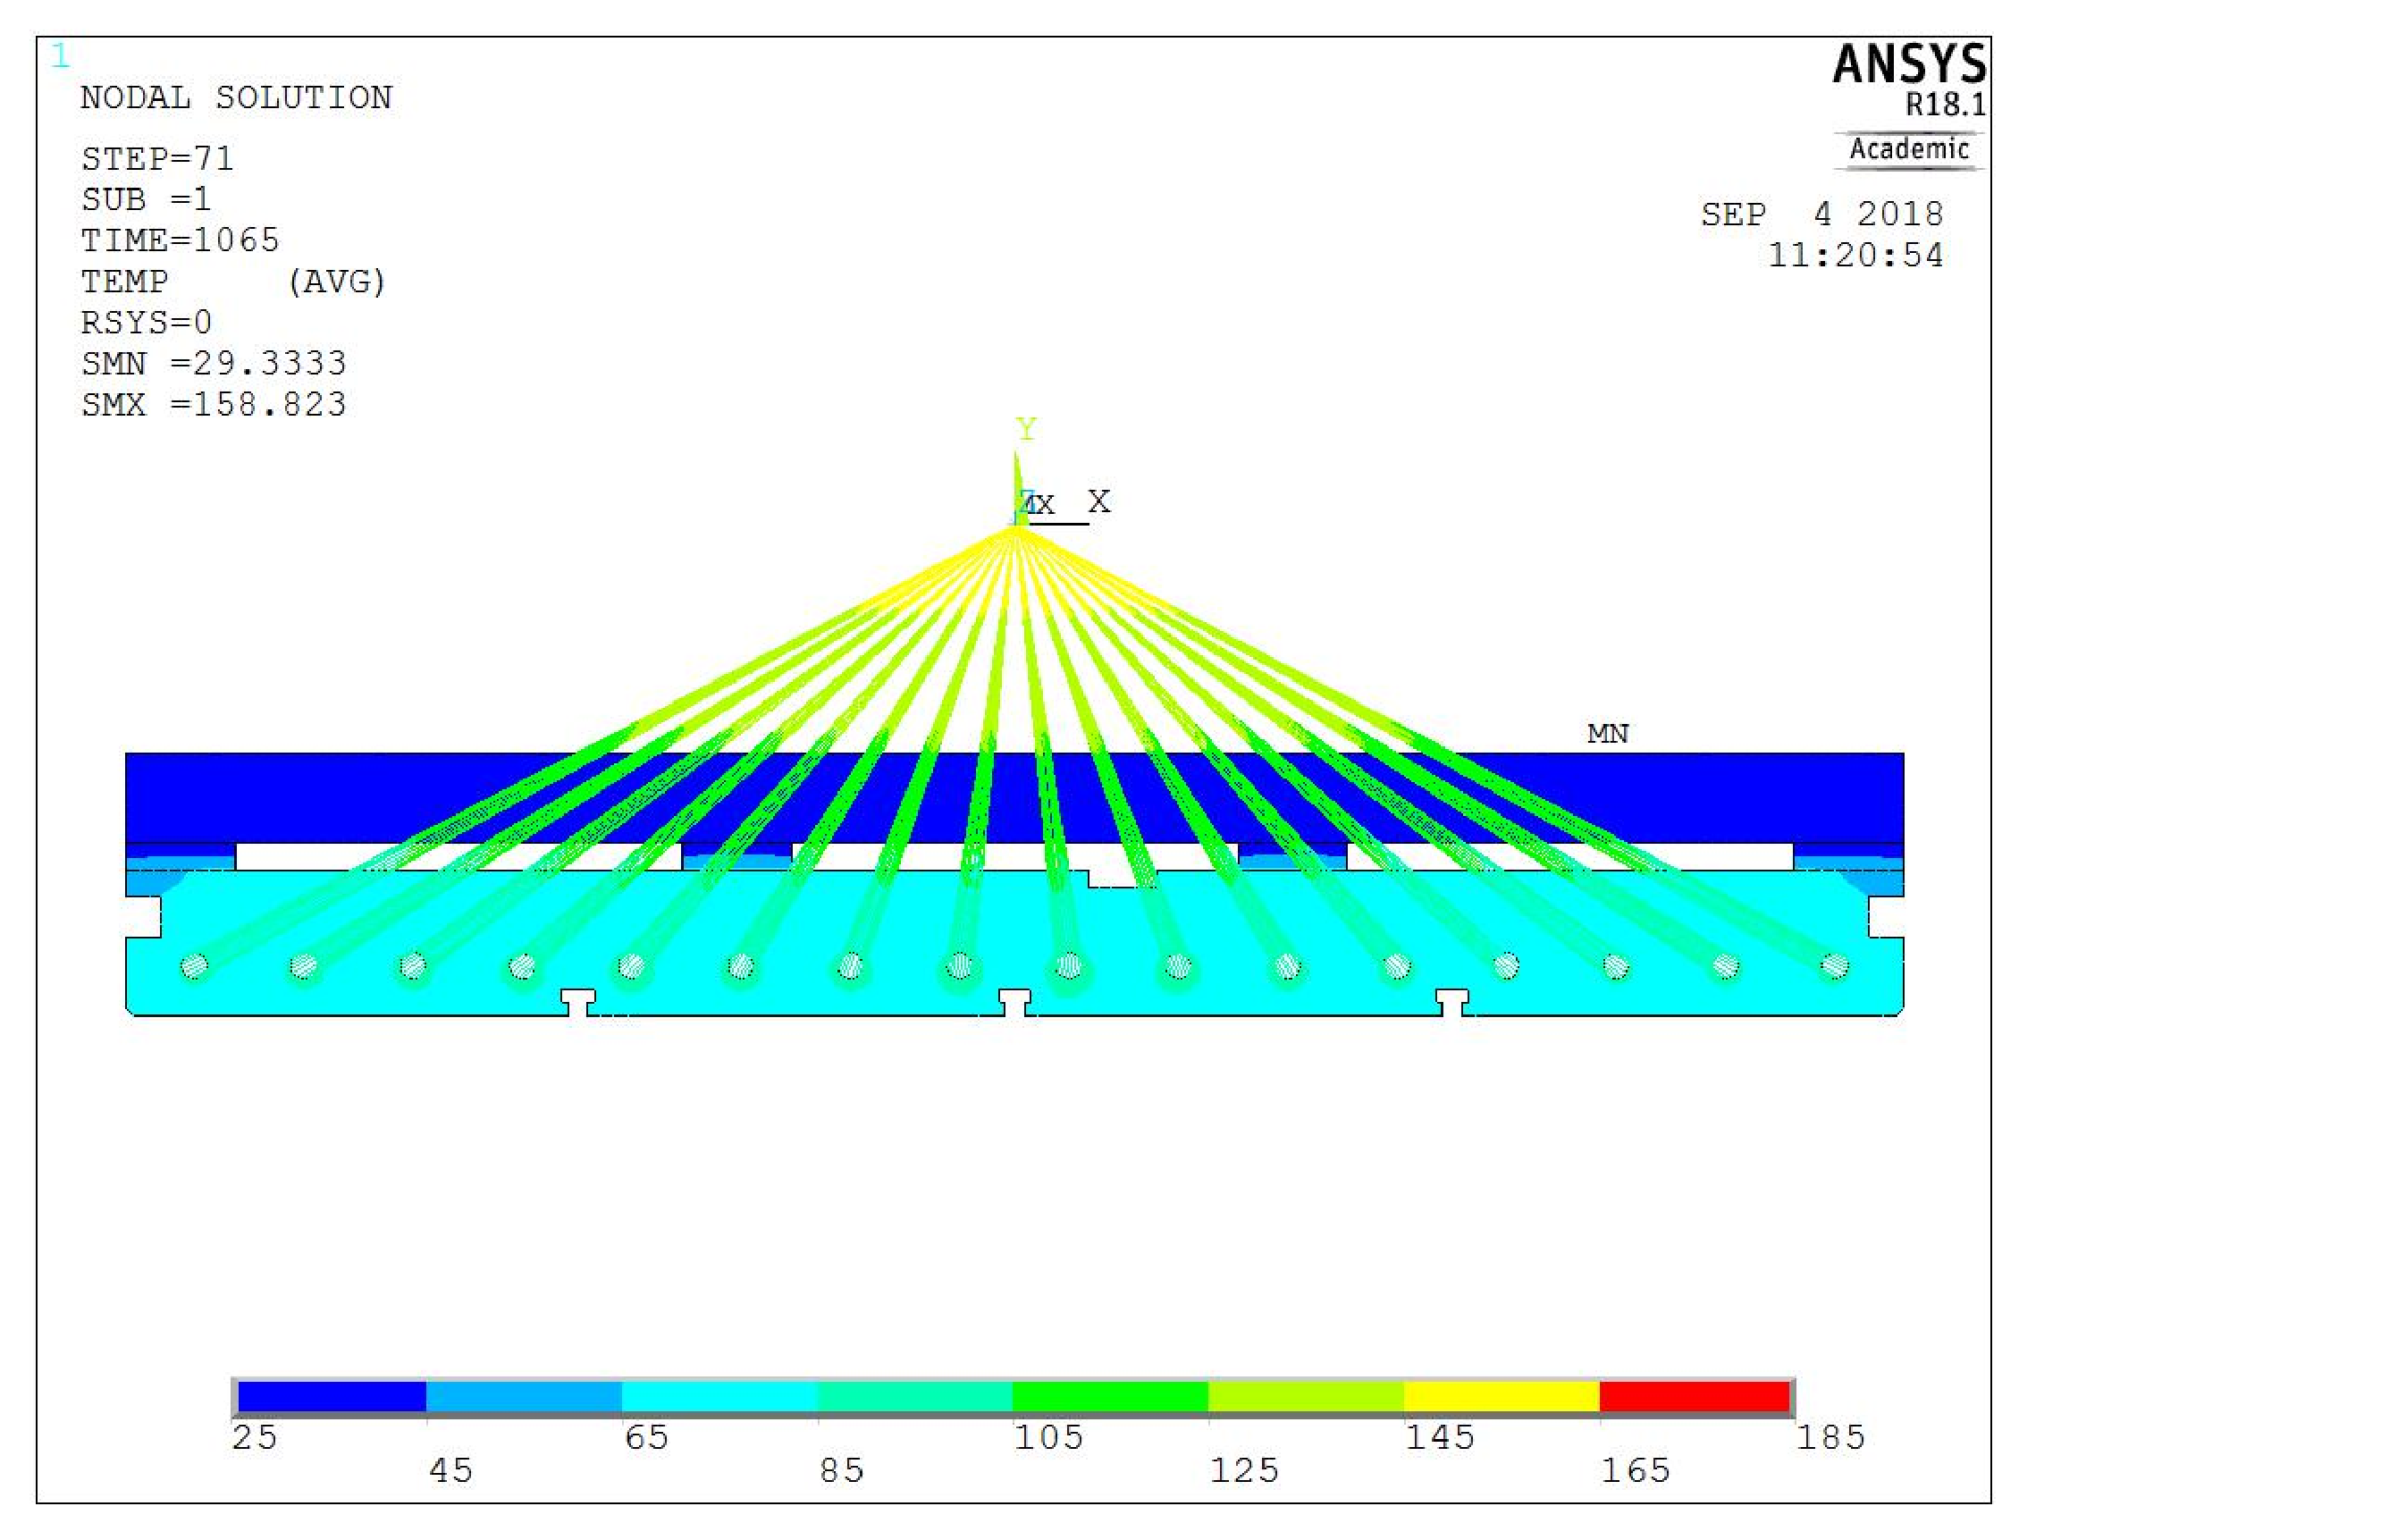
\includegraphics[scale=0.12]{Figures/animation/Figure_9.pdf}
	\end{subfigure}
	\qquad
	\begin{subfigure}[b]{0.25\textwidth}
		\centering
		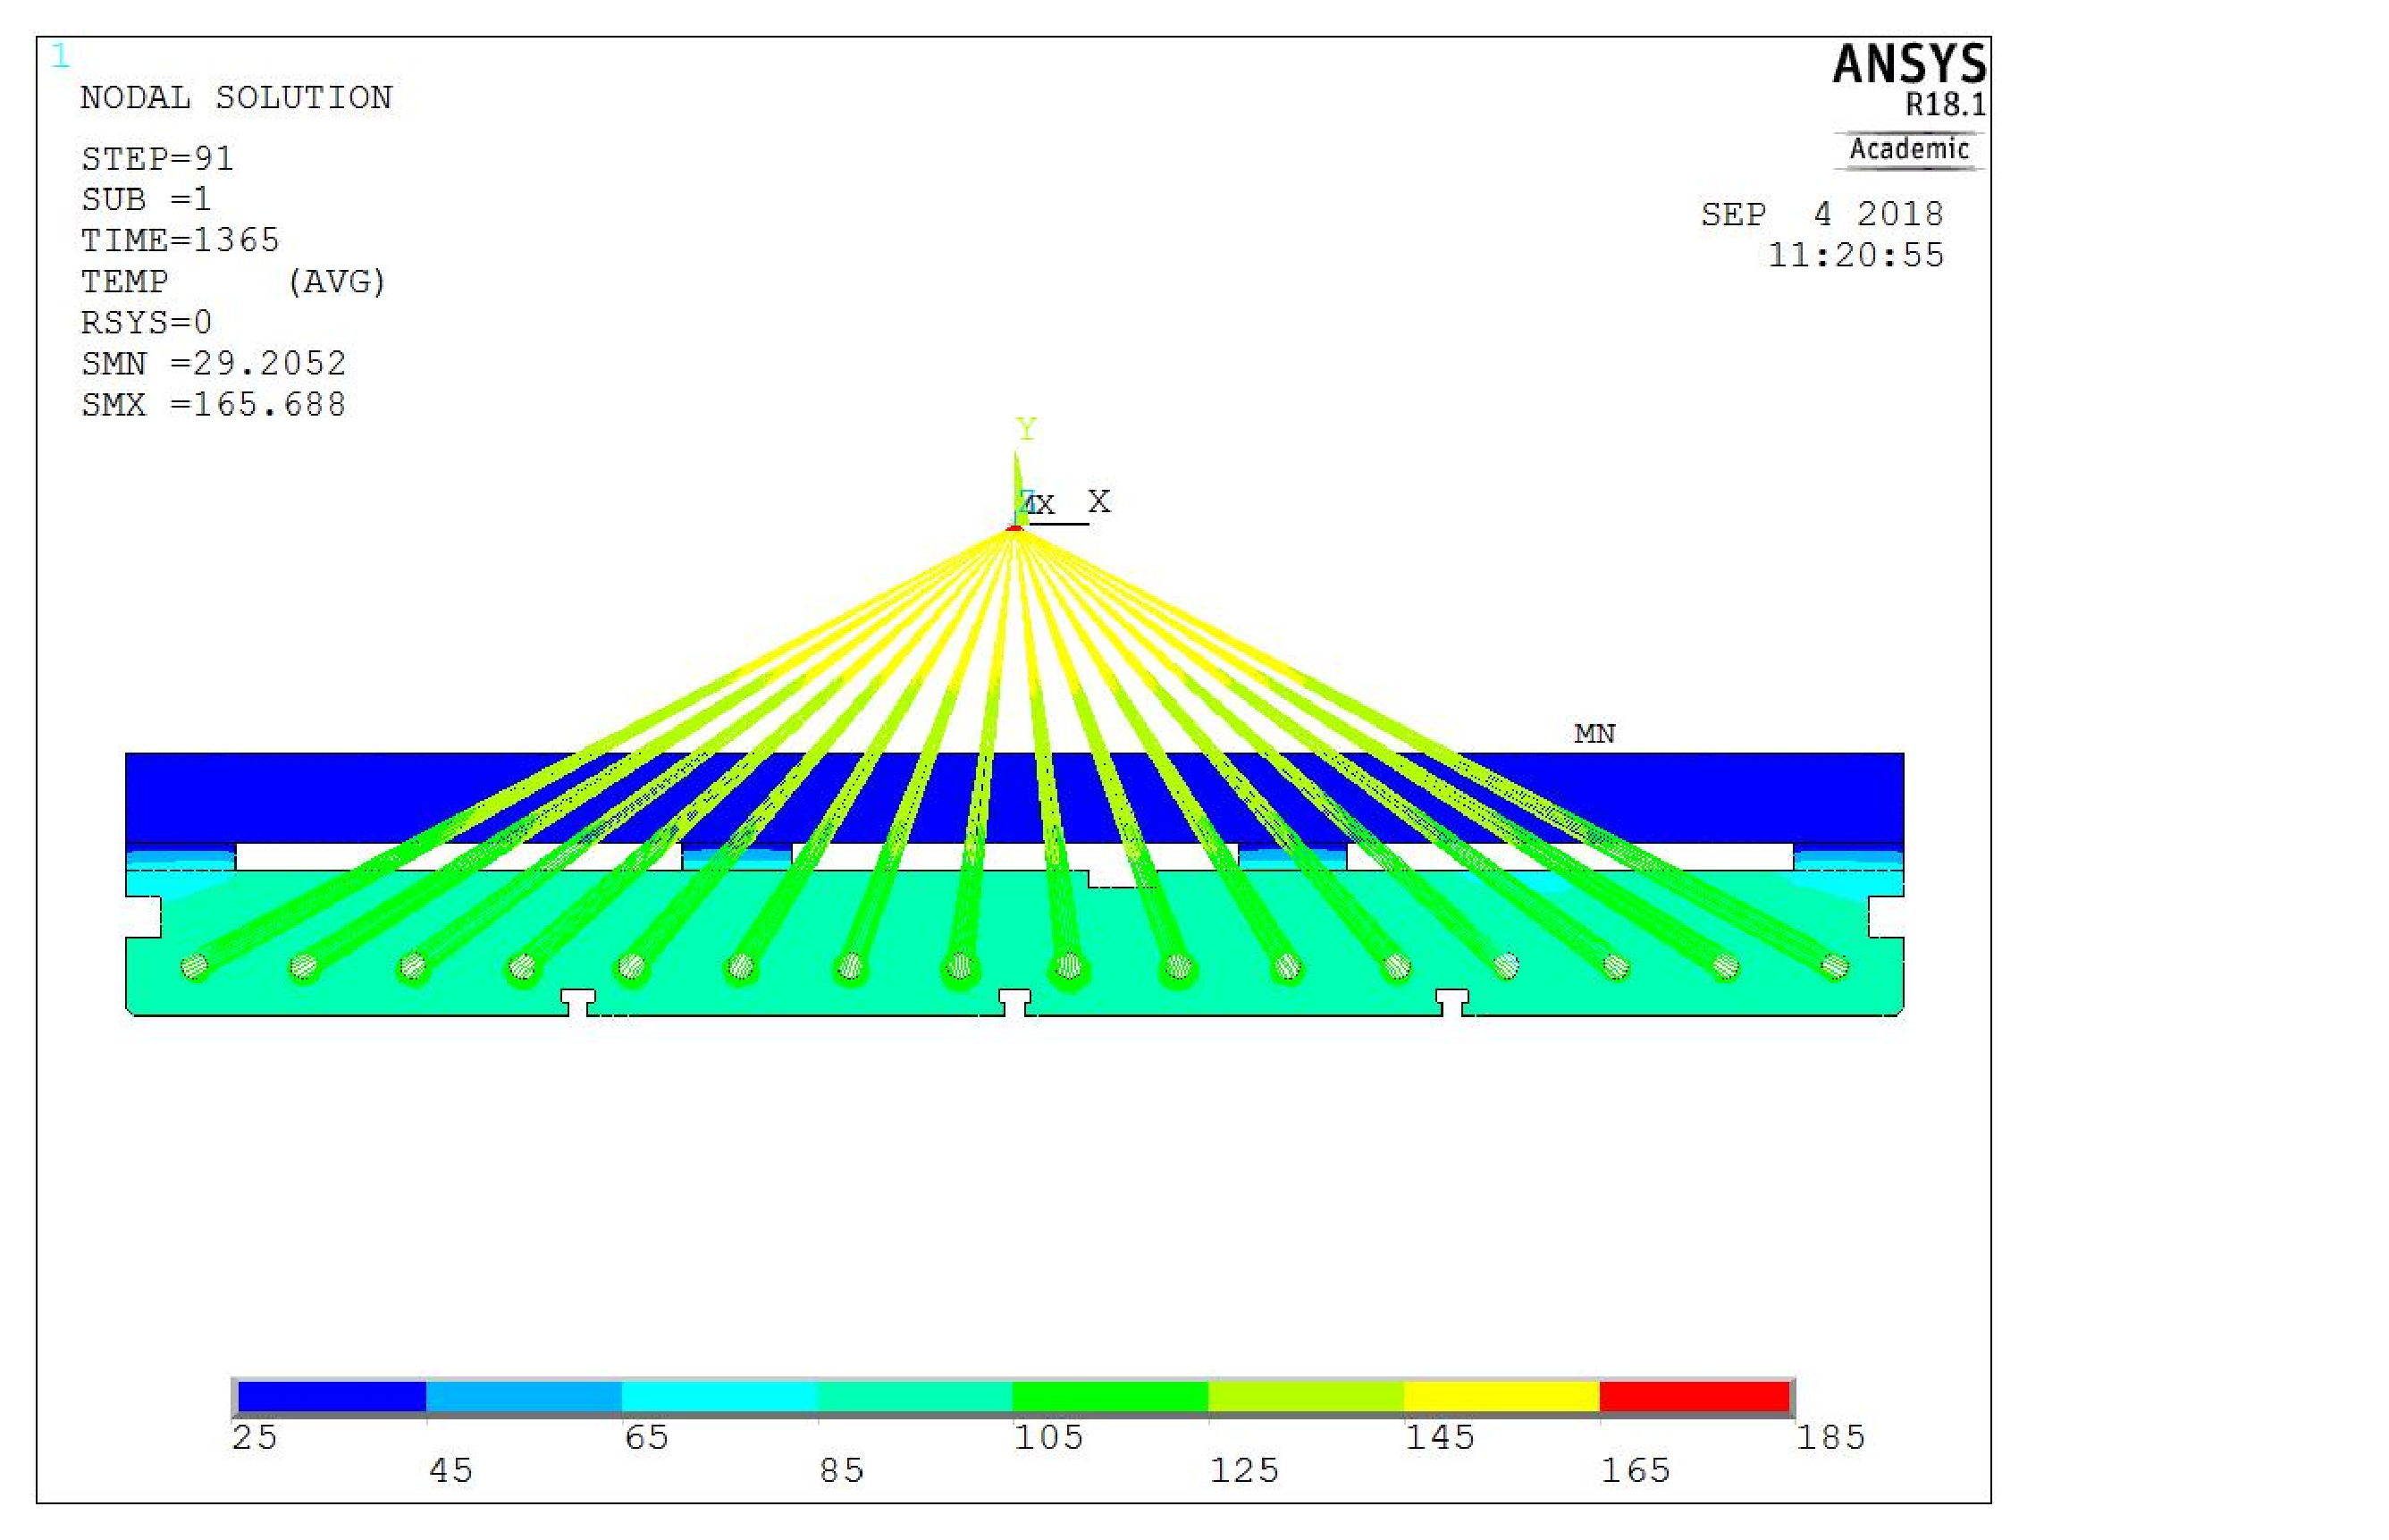
\includegraphics[scale=0.12]{Figures/animation/Figure_11.pdf}
	\end{subfigure}
	\qquad
	\begin{subfigure}[b]{0.25\textwidth}
		\centering
		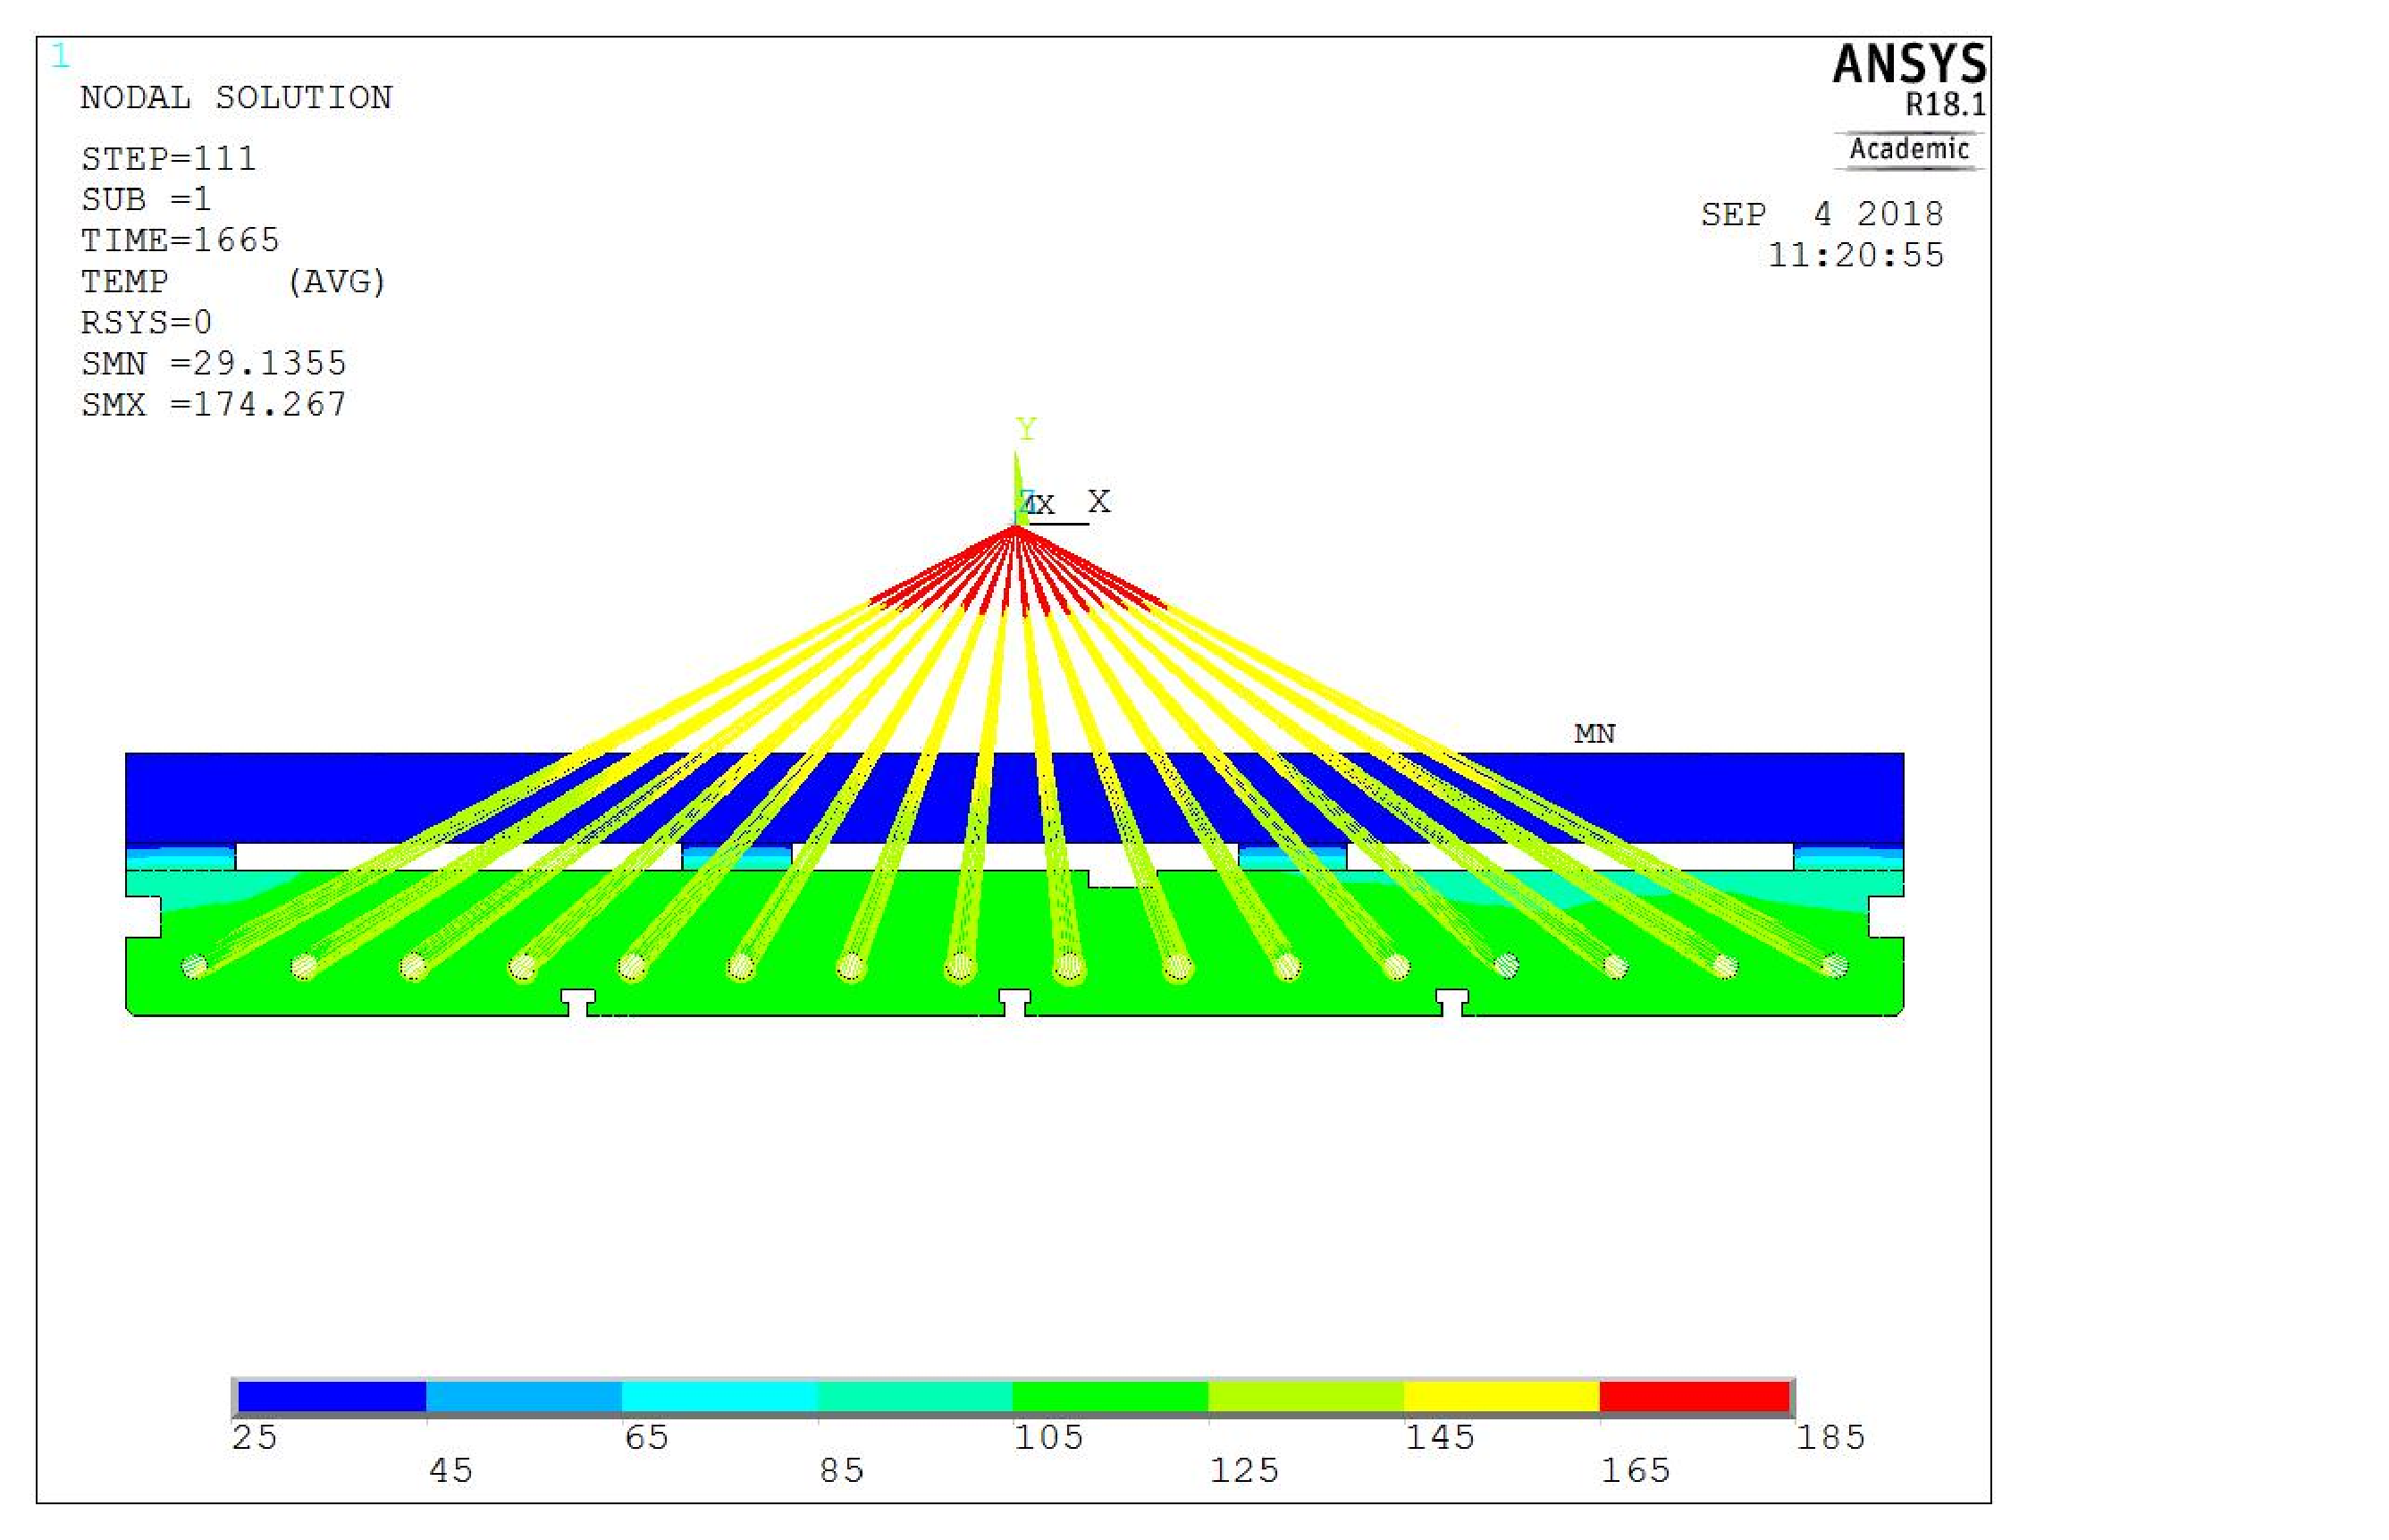
\includegraphics[scale=0.12]{Figures/animation/Figure_13.pdf}
	\end{subfigure}
	\qquad
	\begin{subfigure}[b]{0.25\textwidth}
		\centering
		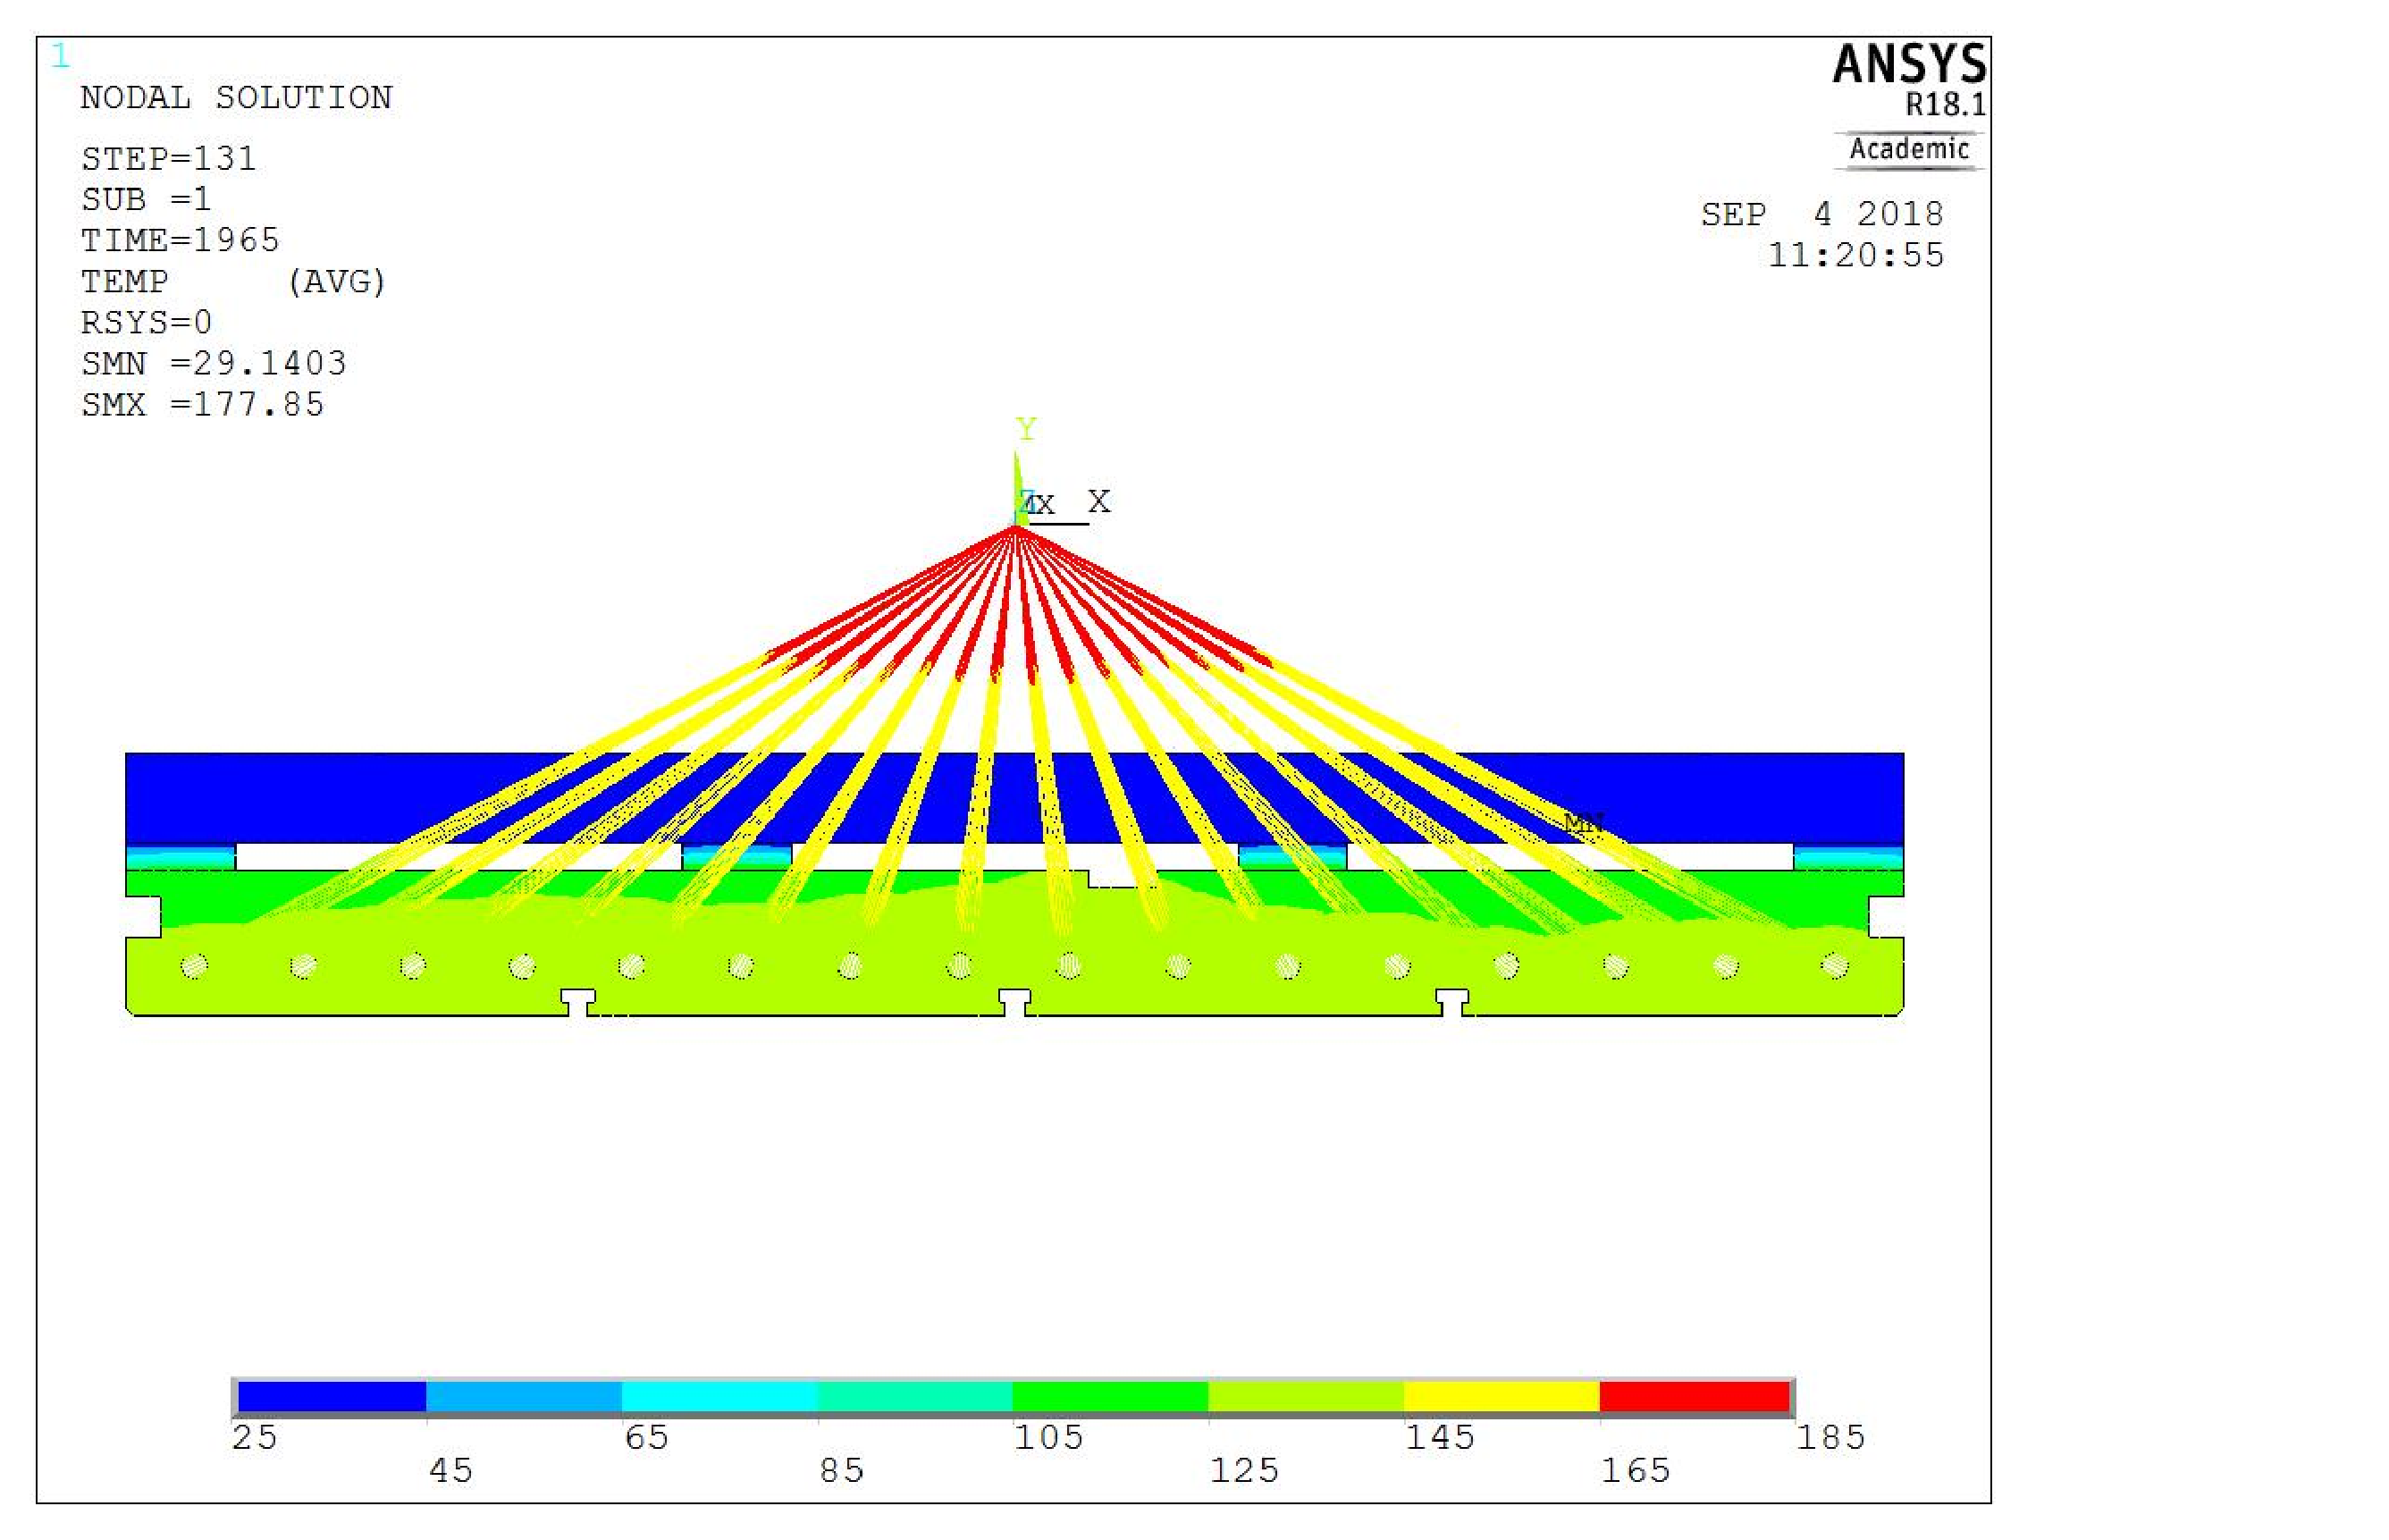
\includegraphics[scale=0.12]{Figures/animation/Figure_15.pdf}
	\end{subfigure}
	\caption{Exemple de figure générées} 
	\label{figure_deux_logo_SYMME}
\end{figure}


\FloatBarrier
%###########################################################################
%###########################################################################

\section{Code \LaTeX}
\subsection{Préparation \LaTeX}
La génération d'animation est possible grâce à l'utilisation du package "animate". Il faut donc ajouter en début de document : \verb|\usepackage{animate}|. Des informations complémentaires sont accessibles sur la \href{http://tug.ctan.org/macros/latex/contrib/animate/animate.pdf}{page de documentation} du package.\\

Ci-dessous, un exemple de code \LaTeX pour la création d'une animation. \\


\verb|\begin{figure}[hbtp]|  \\
\verb|\begin{center}|  \\
\verb|\animategraphics[|  \\
\verb|autoplay, 		% Lecture automatique à l'affichage de la page |  	\\
\verb|loop,				% Boucle de lecture de l'animation |  		\\
\verb|poster=first, |  \\
\verb|height=13cm, 		% Dimension de l'animation |  \\
\verb|width=18cm ,		% Dimension de l'animation |  \\
\verb|controls]{5}{/animation/Figure_}{1}{25} % Animation de l'image 1 à 25 avec 5i/s |  \\
\verb|\caption{Exemple d'animation (Adobe reader 10 minimum requis)} |  \\
\verb|\label{Fig_animation} |  \\
\verb|\end{center} |   \\
\verb|\end{figure}|  \\


\subsection{Avertissement}
Pour le bon fonctionnement de l'animation sur le document pdf final, il est nécessaire de posséder Adobe reader X au minimum. \\

L'impression papier quant à elle est censé faire figuer l'image déterminée par la commande "poster".

\subsection{Exemple d'animation}

Un exemple d'animation est présenté Figure.~\ref{Fig_animation}. \\

Cette animation représente la chauffe d'une structure 2D après l'exécution d'un calcul éléments finis sur le logiciel Ansys. \\


\begin{figure}[hbtp]
\begin{center}
\animategraphics[
autoplay, 
loop,
poster=first,
height=13cm, 
width=18cm ,
controls]{5}{/animation/Figure_}{1}{25}
\caption{Exemple d'animation (Adobe reader 10 minimum requis)} 
\label{Fig_animation} 
\end{center}  
\end{figure}


%%%%%%%%%%%%%%%%%%%%%%%%%%%%%%%%%%%%%%%%%%%%%%%%%%%%%%%%%%%%%%%%%%%%%%%%%%%%%%%%%%%%
%%-------------> FIN DU DOCUMENT
%%%%%%%%%%%%%%%%%%%%%%%%%%%%%%%%%%%%%%%%%%%%%%%%%%%%%%%%%%%%%%%%%%%%%%%%%%%%%%%%%%%%

\end{document}